\section{Evaluation}

In the implementation of the Computation Tree Logic (CTL) bug checker specifications by Abal et. al., the checkers implement four predicates, forming the CTL formula $a\;\text{EU}\;(b\;\land\;EX\;(c\;\text{EU}\;d))$ \cite{Abal2017EffectiveBF}\cite{research-project}. This formula can also be written as $E\;[a\;\cup\;b\;\land\;EX\;E[c\;\cup\;d]]$. This limits the expressiveness of checks which can be defined, given that the logic for detecting bugs must be implemented within these four functions. Specifying the checkers as monitor templates therefore allows for greater expressiveness in the checker definition. To illustrate this, Figure \ref{expressive-monitor} below shows a monitor template definition which cannot be defined in the existing CTL implementation of the EBA framework. 

\begin{figure}[H]
    \centering
    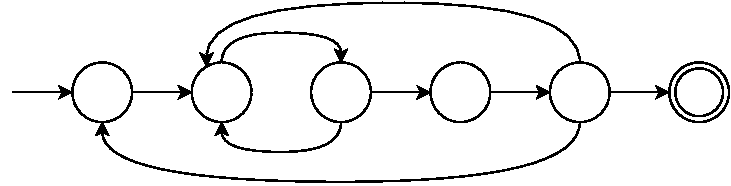
\includegraphics[width=0.5\textwidth]{evaluation/figures/monitor}
    \caption{An illustration of a monitor template which cannot be expressed by the CTL formula $a\;\text{EU}\;(b\;\land\;EX\;(c\;\text{EU}\;d))$.}
    \label{expressive-monitor}
\end{figure}

\newpar On the other hand, the CTL formula $a\;\text{EU}\;(b\;\land\;EX\;(c\;\text{EU}\;d))$ \textit{can} be expressed as a monitor template, as seen in Figure \ref{ctl-as-monitor}. 

\begin{figure}[H]
    \centering
    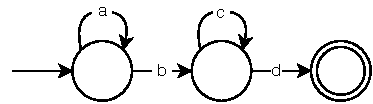
\includegraphics[width=0.35\textwidth]{evaluation/figures/ctl-as-monitor}
    \caption{An illustration of a monitor template equivalent to the CTL formula $a\;\text{EU}\;b\;\text{X}(c\;\text{EU}\;d)$.}
    \label{ctl-as-monitor}
\end{figure}

\newpar This expressiveness allows specifying the CTl checkers defined in the work by Abal et. al and also possible future more granular checkers, in other words increasing the posibilities of extending the EBA framework. Certain bug types can show themselves in different code constructions, such as a double-unlock bug being defined as both an unlock happening before any locks happening and explicit double-unlocks. The expressiveness of monitor templates allows specifying multiple types of behaviour in the code under analysis for a single bug type as more complex transition function in order to increase the precision of checks.

\newpar Experimental static analysis has recently been added to the GCC compiler chain \cite{gcc10}, allowing developers to run check for double-free bugs in their code. David Malcolm --- the developer of the static analysis released in GCC 10 --- has described his challenges in reducing the amount of false positives during the development of the analysis \cite{gcc10-development}, showing that reducing these proves to be a difficult problem. Reducing false positives is important, since developers might avoid using a tool if they see false output too often. The developer of the popular \texttt{curl} command-line tool confirms this, noting that the addition of the analysis in GCC 10 is appreciated, but that it still produces too many false positives to be usable. \cite{curl-static-analysis}. Reducing the amount of false positives in the implementation of monitor templates has been difficult, since a tradeoff between the ability to detect more bugs and reducing the amount of false positives has to be made. In other words, increasing precision is hard. This is reflected in the evaluation of the implementation of monitor templates. We see that the actual bugs are present, but false positives are also reported. 

\begin{table}[H]
    \centering
    \setlength{\tabcolsep}{5pt}
    \scriptsize
    \begin{tabular}{lllll}
    \textbf{File}                                 & \textbf{Present in} & \textbf{My Approach}  & \textbf{Previous Approach} & \textbf{Patched in} \\
    \hline
    drivers/block/drbd/drbd\_main.c               & \texttt{b0814361}            & Detected              & Not detected               & \texttt{8e9c5230}            \\
    fs/ubifs/orphan.c                             & \texttt{7542c6de}            & Detected              & Detected                   & \texttt{4dd75b33}            \\
    drivers/gpu/drm/nouveau/nouveau\_svm.c        & \texttt{5fbcf501}            & Not detected          & Not detected               & \texttt{de4ee728}            \\
    fs/btrfs/file.c                               & \texttt{78e03651}            & Not detected          & Not detected               & \texttt{f49aa1de}            \\
    drivers/staging/wilc1000/wilc\_wlan.c         & \texttt{ca641bae}            & Not detected          & Not detected               & \texttt{fea69916}            \\
    drivers/staging/kpc2000/kpc\_dma/fileops.c    & \texttt{d4c596eb}            & Not detected          & Not detected               & \texttt{c85aa326}            \\
    fs/nfs/client.c                               & \texttt{a46126cc}            & Not detected          & Not detected               & \texttt{c260121a}            \\
    fs/btrfs/file.c                               & \texttt{2b90883c}            & Not detected          & Not detected               & \texttt{8fca9550}            \\
    drivers/media/dvb-core/dvbdev.c               & \texttt{ded71626}            & Internal error        & Internal error             & \texttt{122d0e8d}            \\
    mm/memory\_hotplug.c                          & \texttt{6376360e}            & Detected              & Not detected               & \texttt{e3df4c6e}            \\
    sound/soc/codecs/pcm512x.c                    & \texttt{fd270fca}            & Not detected          & Not detected               & \texttt{28b698b7}            \\
    drivers/target/target\_core\_user.c           & \texttt{807cf197}            & Not detected          & Not detected               & \texttt{f0e89aae}            \\
    drivers/rpmsg/qcom\_smd.c                     & \texttt{fb416f69}            & Not detected          & Not detected               & \texttt{c3388a07}            \\
    drivers/scsi/aacraid/commsup.c                & \texttt{09624645}            & Not detected          & Not detected               & \texttt{d844752e}            \\
    drivers/staging/rtl8188eu/os\_dep/usb\_intf.c & \texttt{612e1c94}            & Compile error         & Compile error              & \texttt{23bf4042}            \\
    block/blk-cgroup.c                            & \texttt{e0223003}            & Compile error         & Compile error              & \texttt{bbb427e3}  
    \end{tabular}
    \caption{The results of comparing the previous CTL-based approach to my monitor-template-based approach.}
    \label{evaluation-table}
\end{table}

\newpar These false positives are mainly reported in loops. The unrolling of loops in EBA is the cause of these false positives, since monitor templates register loops as multiple repetitions of the same effect when an unrolled loop is encountered. In the case of unlocks, any unlock happening within a loop is therefore reported as a double unlock, since that is how the effect-CFG is structured. The existing implementation of EBA by Abal implements the concept of so-called "kill regions" in each bug checker, which will attempt to identify when the memory region being locked or unlocked is being overwritten as part of a loop and ignore this. This might in turn hide actual positives, bugs, in loops.

\begin{itemize}
    \item Possible comparison to BLAST and Cocinelle tools
\end{itemize}